% Lecture Template for ME3050-001-002-Tristan Hill - Spring 2020
% Dynamics Modeling and Controls
% Time Response - Lecture 3

% I am finally converting my stuff to BEAMER

% Document settings

%\documentclass{beamer}                  % for presentation ?
\documentclass[handout]{beamer}  % for handout ?
\usepackage{beamerthemesplit}
\usepackage{amsmath}
\usepackage{listings}
\usepackage{multicol}

\beamertemplateballitem

\definecolor{TTUpurple}{rgb}{0.3098, 0.1607, 0.5176} % TTU Purple (primary)
\definecolor{TTUgold}{rgb}{1.0000, 0.8666, 0.0000} % TTU Gold (primary)

\setbeamercolor{palette primary}{bg=TTUpurple,fg=TTUgold}
\setbeamercolor{palette secondary}{bg=black,fg=TTUgold}
\setbeamercolor{palette tertiary}{bg=black,fg=TTUpurple}
\setbeamercolor{palette quaternary}{bg=TTUgold,fg=black}
\setbeamercolor{structure}{fg=TTUpurple} % itemize, enumerate, etc
\setbeamercolor{section in toc}{fg=TTUpurple} % TOC sections

%\usefonttheme{professionalfonts}

\newcommand{\LNUM}{3\hspace{2mm}} % Lecture Number 

\newcommand{\vspcc}{\vspace{6mm}\\ } 
\newcommand{\vspc}{\vspace{3mm}\\ } 
\newcommand{\hspc}{\hspace{5mm} } 

\newcommand{\Lagr}{\mathcal{L}} % lagrangian

\newcommand{\secondtitle}{Step Response of Second Order Systems}% second line of the title of this presentation , aka the topic of this lecture

\title{Time Response - Lecture \LNUM}
\author{ME3050 - Dynamics Modeling and Controls} % original formatting from Mike Renfro, September 21, 2004

\date{March 25, 2020}

\begin{document}

\lstset{language=MATLAB,basicstyle=\ttfamily\small,showstringspaces=false}

% Title page1 
\frame{\titlepage \center\textbf{\secondtitle}\vspcc}


% Section 0: Outline
\frame{

\large \textbf{Lecture \LNUM - \secondtitle} \vspc

 \begin{itemize}

	\item The Step Input\vspc % Section 1

	\item Response Equations for Three Cases\vspc        % Section 2
	
	\item Description and Specification of The Step Response\vspc %Section 3

	\item Affect of Root Location on Response \vspc % Section 4

\end{itemize}

}


%Section 1: Forced Response of a Second Order Model % I think this section goes in the next lecture... 
\section{ The Step Input}

\frame{
\frametitle{The Step Input}

\large Now, consider the mass-spring system with damping present subject to {\bf step} input. This models instantly turning on the input force $f(t)$.\vspc

\begin{multicols}{2}

	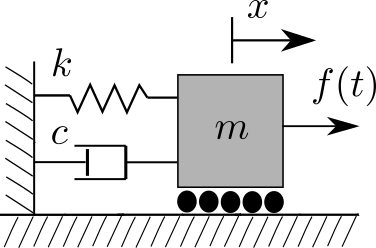
\includegraphics[scale=.4]{mass_spring_04.png} \hspc  

	\underline{Heavyside's Step Function}\vspc
	\[f(t) = \begin{cases} 
	      0 & t < 0 \\
	      F & t\geq 0 \\
	   \end{cases}
	\]\\

\end{multicols}

\large The EOM is:\vspc

	\scalebox{1.0}{$m\ddot{x} +c\dot{x}+kx=f(t)$\hspace{3mm}with\hspace{3mm}$x(t=0)=x_0$\hspace{3mm}and\hspace{3mm}$v(t=0)=v_0$}\vspc

}



% section 2: Response Equations for Three Cases

\section{Response Equations for Three Cases}

\subsection{Complementary Part of Solution}
\frame{
\frametitle{Complementary Part of Solution}
The free response equations derived in the previous lecture represent the {\it comlpementary part} of the solution. We also need to find the {\it particular part} to see the step response of the system. \vspcc

Once again, the solution takes one of three forms. The response equations for each are in your reference handout. \vspcc


}

\subsection{The Overdamped Case}
\frame{
\frametitle{The Overdamped Case}

\large \underline{Overdamped}\hspc $c>2\sqrt{mk} \hspc \implies\hspc \zeta>1$ \hspc \vspcc

roots: \scalebox{1}{$s_{1,2}=-\zeta\omega_n\pm\omega_n\sqrt{\zeta^2-1}$} \vspcc

\scalebox{1}{$x(t)=C_1e^{-s_1t}+C_2^{-s_2t}+\frac{F}{K}$} \vspcc

The {\it unit step response} is found with zero initial conditions $x_0=0$\hspace{3mm}$v_0=0$ and a unit step input $F=1$.    \vspcc

\scalebox{1}{$x(t)=\frac{1}{K}(\frac{s_2}{s_1-s_2}e^{-s_1t}-\frac{s_1}{s_1-s_2}e^{-s_2t}+1)$}

}

\subsection{The Critically Damped Case}
\frame{
\frametitle{The Critically Damped Case}

\large \underline{Critically Damped}\hspc $c=2\sqrt{mk} \hspc \implies\hspc \zeta=1$ \hspc \vspcc

roots: \scalebox{1}{$s_{1,2}=\frac{-c}{2m}=\zeta\omega_n=-\omega_n$}\vspc

\scalebox{1}{$x(t)=C_1e^{-\omega_nt}+C_2te^{-\omega_nt}+\frac{F}{K}=(C_1+C_2t)e^{-\omega_nt}+\frac{F}{K}$}\vspcc

The {\it unit step response} is found with zero initial conditions $x_0=0$\hspace{3mm}$v_0=0$ and a unit step input $F=1$.    \vspcc

\scalebox{1}{$x(t)=\frac{1}{K}[(-1-\omega_nt)e^{-\omega_nt}+1]$}

}

\subsection{The Underdamped Case}
\frame{
\frametitle{The Underdamped Case}

\large \underline{Underdamped}\hspc $c<2\sqrt{mk} \hspc \implies\hspc \zeta<1$ \hspc \vspcc

\scalebox{1}{$s_{1,2}=-\zeta\omega_n\pm j\omega_d$}\vspc

\scalebox{1}{$x(t)=C_1e^{-\zeta\omega_nt}sin(\omega_dt+\phi)+\frac{F}{K}$}\vspc

The {\it unit step response} is found with zero initial conditions $x_0=0$\hspace{3mm}$v_0=0$ and a unit step input $F=1$.    \vspcc

\scalebox{1}{$x(t)=\frac{1}{K}\left[\frac{1}{\sqrt{1-\zeta^2}}e^{-\zeta\omega_nt}sin(\omega_dt+\phi)+1\right]$}\vspc
\scalebox{1}{$\phi=tan^{-1}\left(\frac{\sqrt{1-\zeta^2}}{\zeta}\right)+\pi$}\vspc

}

\subsection{}
\frame{
\frametitle{Unit Step Response}
The {\bf unit step response} is a special case of the {\it forced response} in which $f(t)$ is the step function of magnitude 1. \vspcc
\renewcommand{\arraystretch}{2}
\begin{tabular}{|c|c|}
Overdamped&\scalebox{1}{$x(t)=\frac{1}{K}(\frac{s_2}{s_1-s_2}e^{-s_1t}-\frac{s_1}{s_1-s_2}e^{-s_2t}+1)$}\\
Critically Damped&\scalebox{1}{$x(t)=\frac{1}{K}[(-1-\omega_nt)e^{-\omega_nt}+1]$}\\
Underdamped&\scalebox{1}{$x(t)=\frac{1}{K}\left[\frac{1}{\sqrt{1-\zeta^2}}e^{-\zeta\omega_nt}sin(\omega_dt+\phi)+1\right]$}\\
&\scalebox{1}{$\phi=tan^{-1}\left(\frac{\sqrt{1-\zeta^2}}{\zeta}\right)+\pi$}\\
\end{tabular}

}


%Section 3: Description and Specification of System Response
\section{Description and Specification of System Response}
\frame{
\frametitle{Description and Specification of System Response}

We are going to derive several quatities that describes the response of an underdamped system. \vspc

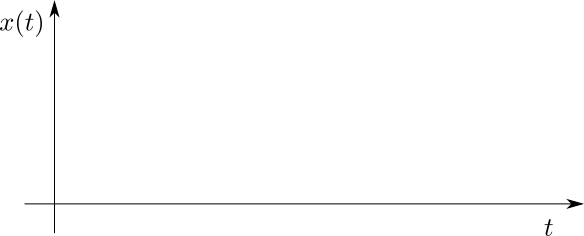
\includegraphics[scale=0.7]{lecture3_fig1.png}

}

\subsection{Rise Time}
\frame{
\frametitle{Rise Time}

The {\bf rise time} is the time at which the response first equals the steady state value.\vspc

%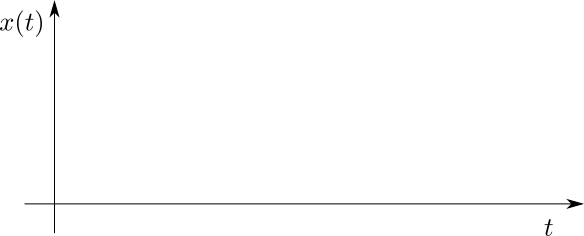
\includegraphics[scale=0.35]{lecture3_fig1.png}\vspc
\scalebox{1}{$x(t)=\frac{1}{K}\left[\frac{1}{\sqrt{1-\zeta^2}}e^{-\zeta\omega_nt}sin(\omega_dt+\phi)+1\right]$}\vspc

Set the {\it transient term} to zero and solve for $t$.\vspc
\scalebox{1}{$e^{-\zeta\omega_nt}sin(\omega_dt+\phi)=0\implies sin(\omega_dt+\phi)=0\implies \omega_dt+\phi=2\pi$}\vspc
\scalebox{1.25}{$t_{rise}=t_r=\frac{2\pi-\phi}{\omega_d}$}

}

\subsection{Peak Time}
\frame{
\frametitle{Peak Time}

The {\bf peak time} is the time at which the response equals the maximum value. Find the derivative of the response equation and set it equal to zero. \vspc

\scalebox{1}{$\dot{x}(t)=$}\vspc
\scalebox{1}{$\left(\frac{1}{K}\frac{1}{\sqrt{1-\zeta^2}}\right)\left[ e^{-\zeta\omega_nt}(\omega_dcos(\omega_dt+\phi))+sin(\omega_dt+\phi)(-\zeta\omega_ne^{-\zeta\omega_nt})\right]$} \vspc
%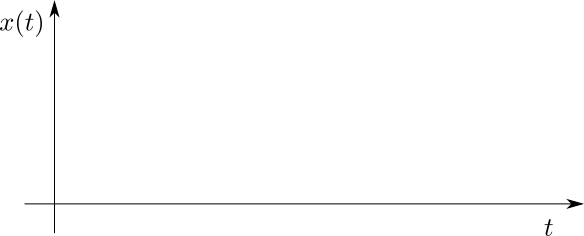
\includegraphics[scale=0.7]{lecture3_fig1.png}
\scalebox{1}{$sin(\omega_d)t=0\implies \omega_dt=\pi\implies$}\scalebox{1.25}{$ t_{peak}= t_p=\frac{\pi}{\omega_d}$}\vspc

}
\subsection{Settling Time}
\frame{
\frametitle{Settling Time}

The {\bf settling time} is the time at which the response decays to a certain percentage of the steady state value.\vspc

It can be esitmated as:\vspc
\scalebox{1.25}{$t_{settling}=t_s=-\frac{ln(tolerance)}{\zeta\omega_n}$}\vspc

\scalebox{1}{$2\%\implies tolerance=0.02$}\vspc
\scalebox{1}{$5\%\implies tolerance=0.05$}\vspc
%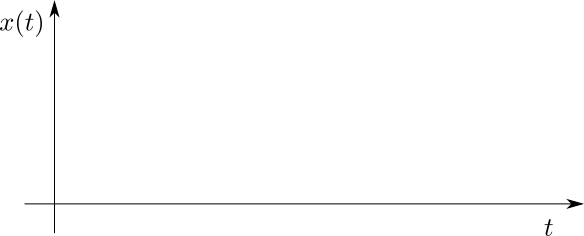
\includegraphics[scale=0.7]{lecture3_fig1.png}

}


\subsection{Maximum Overshoot}
\frame{
\frametitle{Maximum Overshoot}

The {\bf maximum overshoot} is the response beyond the steady state value. \vspc

\scalebox{1.0}{$M_p=x(t_p)-x_{ss}\implies M_p=\frac{1}{K}e^{\frac{-\pi\zeta}{\sqrt{1-\zeta^2}}}$}\vspcc

This is often expressed as a percentage. \vspc

\scalebox{1.25}{$M_\%=\frac{x(t_p)-x_{ss}}{x_{ss}}100=100e^{\frac{-\pi\zeta}{\sqrt{1-\zeta^2}}}$}

%=100e^{-\frac{\pi\zeta}{\sqrt{1-\zeta^2}}}$}
%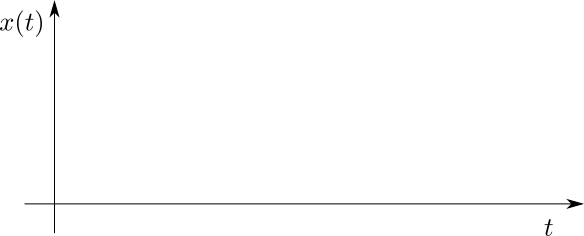
\includegraphics[scale=0.7]{lecture3_fig1.png}

}

\frame{
\frametitle{Damping Ratio from Maximum Overshoot}

The {\it damping ratio} can be determined from the maximum overshoot! \vspc

\scalebox{1}{$M_\%=100e^{\frac{-\pi\zeta}{\sqrt{1-\zeta^2}}}$}\vspc

Solve for $\zeta$.\vspc

\scalebox{1}{$\zeta=\frac{R}{\sqrt{\pi^2+R^2}}$\hspc with\hspc$R=ln\left(\frac{100}{M\%}\right)$}\vspc

}


% Section 4: Affect of Root Location on Response
\section{Affect of Root Location on Response}
\frame{
\frametitle{Affect of Root Location on Response}
 	
	The {\it location} of the root in the {\it complex plane} shows the affects of the roots on the system behviour.\vspc
	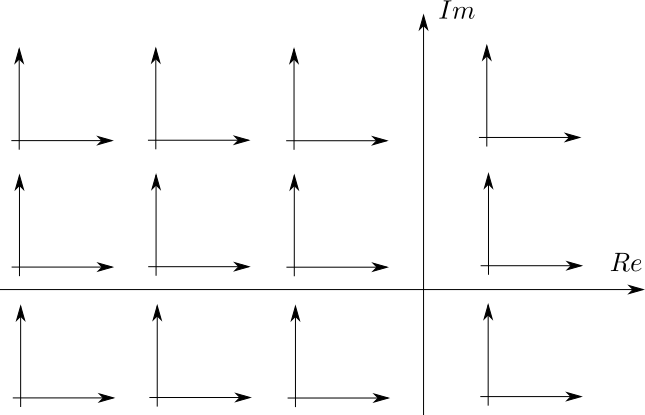
\includegraphics[scale=0.4]{lecture3_fig5.png}

}

\frame{
\frametitle{Along a Vertical Line}
 	
	As the root moves along a vertical line...\vspc
	
\includegraphics[scale=0.5]{lecture3_fig2.png}

}
\frame{
\frametitle{Along a Horizontal Line}
 	
	As the root moves along a horizontal line...\vspc
	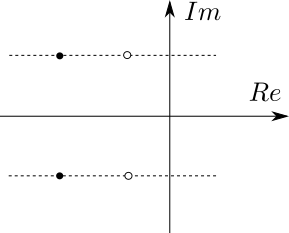
\includegraphics[scale=0.5]{lecture3_fig3.png}

}
\frame{
\frametitle{Along a Diagonal Line}
 	
	As the root moves along a diagonal line...\vspc
	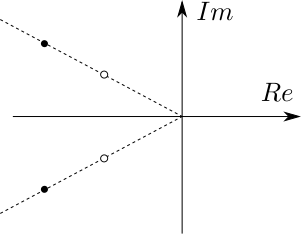
\includegraphics[scale=0.5]{lecture3_fig4.png}

}

% references is not a section for now, for looks and it would be a waste of space
\frame{

\frametitle{References}

\begin{itemize}
	\item System Dynamics, Palm III, Third Edition - Section 8.3 - Step Response of Second Order Systems
\end{itemize}

}
\end{document}









 